\documentclass[aspectratio=169, journal, x11names, unknownkeysallowed, hyperref={colorlinks,
linkcolor = SS2,
urlcolor  = F3,
citecolor = F3,
anchorcolor = A4}, 12pt]{beamer}
%\usepackage{movie15}

\usepackage[utf8]{inputenc} 
\usepackage{lmodern}
\setbeamertemplate{navigation symbols}{}
\usepackage[english]{babel}
\usepackage{booktabs}%toprule middlerule bottomrule
\usepackage{subfigure}%several picture in one frame
\usepackage{fontawesome}
\usepackage{amsmath,amsfonts,amssymb}
\usepackage{multimedia}
\usepackage{tikz}
\usetikzlibrary{shapes.geometric, arrows, calc}
\usepackage{svg}
\usepackage{xcolor}
\usepackage{chemfig}
\usepackage{graphicx}
\usepackage{colortbl}
\usepackage{appendixnumberbeamer}
\usepackage{pifont}
\usepackage[absolute,overlay]{textpos}
\usepackage{multirow, cellspace}
\usepackage[final]{pdfpages}
\usepackage[skins]{tcolorbox}
\usepackage{listings}
\usepackage{pdfpages}
\usepackage[backend=biber, style=authoryear-comp, sorting=nyt, url=false, isbn=false, doi=false, clearlang=false, maxbibnames=10, maxcitenames=2]{biblatex}
\addbibresource{../library.bib}


%\definecolor{shadecolor}{RGB}{239, 239, 239}
\newenvironment{Shaded}{\begin{snugshade}}{\end{snugshade}}
% ---- Color scheme based on https://github.com/arcticicestudio/nord
% - Polar Night
\definecolor{PN0}{RGB}{64,52,64}
\definecolor{PN1}{RGB}{59,66,82}
\definecolor{PN2}{RGB}{67,76,94}
\definecolor{PN3}{RGB}{76,86,106}

% - Snow Storm
\definecolor{SS0}{RGB}{216,222,233}
\definecolor{SS1}{RGB}{229,233,240}
\definecolor{SS2}{RGB}{236,239,244}

% - Frost
\definecolor{F0}{RGB}{143,188,187}
\definecolor{F1}{RGB}{136,192,208}
\definecolor{F2}{RGB}{129,161,193}
\definecolor{F3}{RGB}{94,129,172}

% - Aurora
\definecolor{A0}{RGB}{191,97,106}
\definecolor{A1}{RGB}{208,135,112}
\definecolor{A2}{RGB}{235,203,139}
\definecolor{A3}{RGB}{163,190,140}
\definecolor{A4}{RGB}{180,142,173}

 
\usetheme[compress]{Dresden} %CambridgeUS

\setbeamertemplate{block}[shadow=true] 
\setbeamertemplate{blocks}[rounded][shadow=false]
\setbeamercolor*{block title}{bg=PN3}
\setbeamercolor*{block body}{bg=white!50!gray}
\setlength{\parindent}{0pt}
%\fboxrule=4pt%border thickness

\usecolortheme[named= PN3]{structure}

\setbeamercolor*{author in head/foot}{fg=white,bg=PN1!90}
\setbeamercolor*{title in head/foot}{fg=white,bg=PN3!90}
\setbeamercolor*{section in head/foot}{bg=PN1,fg=white}
\setbeamercolor*{subsection in head/foot}{bg=PN2,fg=white}
\setbeamercolor*{title}{fg=white,bg=PN3}
\setbeamercolor*{frametitle}{fg=white,bg=PN3!80}
\setbeamerfont{page number in head/foot}{size=\scriptsize}

\setbeamertemplate{footline}
{
\pgfdeclarelayer{background}
\pgfdeclarelayer{foreground}
\pgfsetlayers{background,main,foreground}
\begin{tikzpicture}
\\
\begin{pgfonlayer}{background}
\hspace*{0.5cm}
%\includegraphics[width=\textwidth, opacity = 0.8]{Template-Images/Theme/Rahmen_Seitenzahl.png}
\end{pgfonlayer}
\node[color=PN0] (pagenumber) at (15,0.25) {\footnotesize{ { \insertframenumber
  /\inserttotalframenumber}}};
\end{tikzpicture}
}
\defbeamertemplate*{title page}{customized}[1][]
{
\pgfdeclarelayer{background}
\pgfdeclarelayer{foreground}
\pgfsetlayers{background,main,foreground}

\usebeamerfont{institute}\insertinstitute\par
\bigskip
\bigskip
  \usebeamerfont{title}\inserttitle\par  
  \bigskip
  \usebeamerfont{author}\insertauthor\par
  \smallskip
  \usebeamerfont{date}\insertdate\par
  \usebeamercolor[bg]{titlegraphic}\inserttitlegraphic
}

\setbeamertemplate{caption}[]
\useoutertheme{default} %Äußere Themen spezifizieren die Grenzen einer Folie und sagen ob und wo die inneren Elemente liegen.

\setbeamertemplate{enumerate items}[circle]
\setbeamertemplate{itemize items}[circle]
\setbeamerfont{frametitle}{size=\tiny}
\setbeamertemplate{frametitle}{%
    \nointerlineskip%
    \begin{beamercolorbox}[wd=\paperwidth,ht=2.5ex,dp=1ex]{frametitle}
        \hspace*{3ex}\insertframetitle%
    \end{beamercolorbox}%
}
\setbeamersize{text margin left = 1.5em, text margin right = 1.5em}

\newcommand{\backupbegin}{
   \newcounter{finalframe}
   \setcounter{finalframe}{\value{framenumber}}
}
\newcommand{\backupend}{
   \setcounter{framenumber}{\value{finalframe}}
}

\newcommand{\tabitem}{~~\llap{\textbullet}~~}
\newcommand{\oarrow}{\textcolor{A1}{$\rightarrow$} }
\newcommand{\rarrow}{\textcolor{A0}{$\rightarrow$} }
\newcommand{\garrow}{\textcolor{F1}{$\rightarrow$} }

\definecolor{light-gray}{gray}{0.95}

\lstset{language=R,
    basicstyle=\fontsize{6}{9}\selectfont\ttfamily,
    backgroundcolor = \color{light-gray},
    %stringstyle=\color{F3},
    %otherkeywords={0,1,2,3,4,5,6,7,8,9},
    %morekeywords={TRUE,FALSE},
    deletekeywords={data,frame,length,as,character},
    %keywordstyle=\color{A1},
    commentstyle=\color{PN3},
    showstringspaces=false,
    rulecolor=\color{black},
    frameshape={RYR}{Y}{Y}{RYR}
}


\begin{document}
%\renewcommand{\inserttotalframenumber}{5} Ausklammern falls kein Appendix vorhanden
\institute[IRTG] {
\begin{minipage}{\textwidth}
\vspace{-15em}
\hspace*{31em}
%\includegraphics[scale=0.3]{Template-Images/Logos/Signet2018-RGB.png}
\hspace{1em}
%\includegraphics[scale=0.2]{Template-Images/Logos/IFZO.png}
\end{minipage}
}

\title[Research Data Management]{
  \vspace*{-5em} 
\textbf{Data Science für Geistes- und Sozialwissenschaftler} \linebreak  Thema: Regressionsanalyse
}

\author[Me]{\footnotesize\textcolor{PN3}{Martin Kerntopf} \linebreak \textbf{25. Januar 2022}} 
\date{}

%\titlegraphic{\hspace*{-1.2cm} \vspace*{8cm}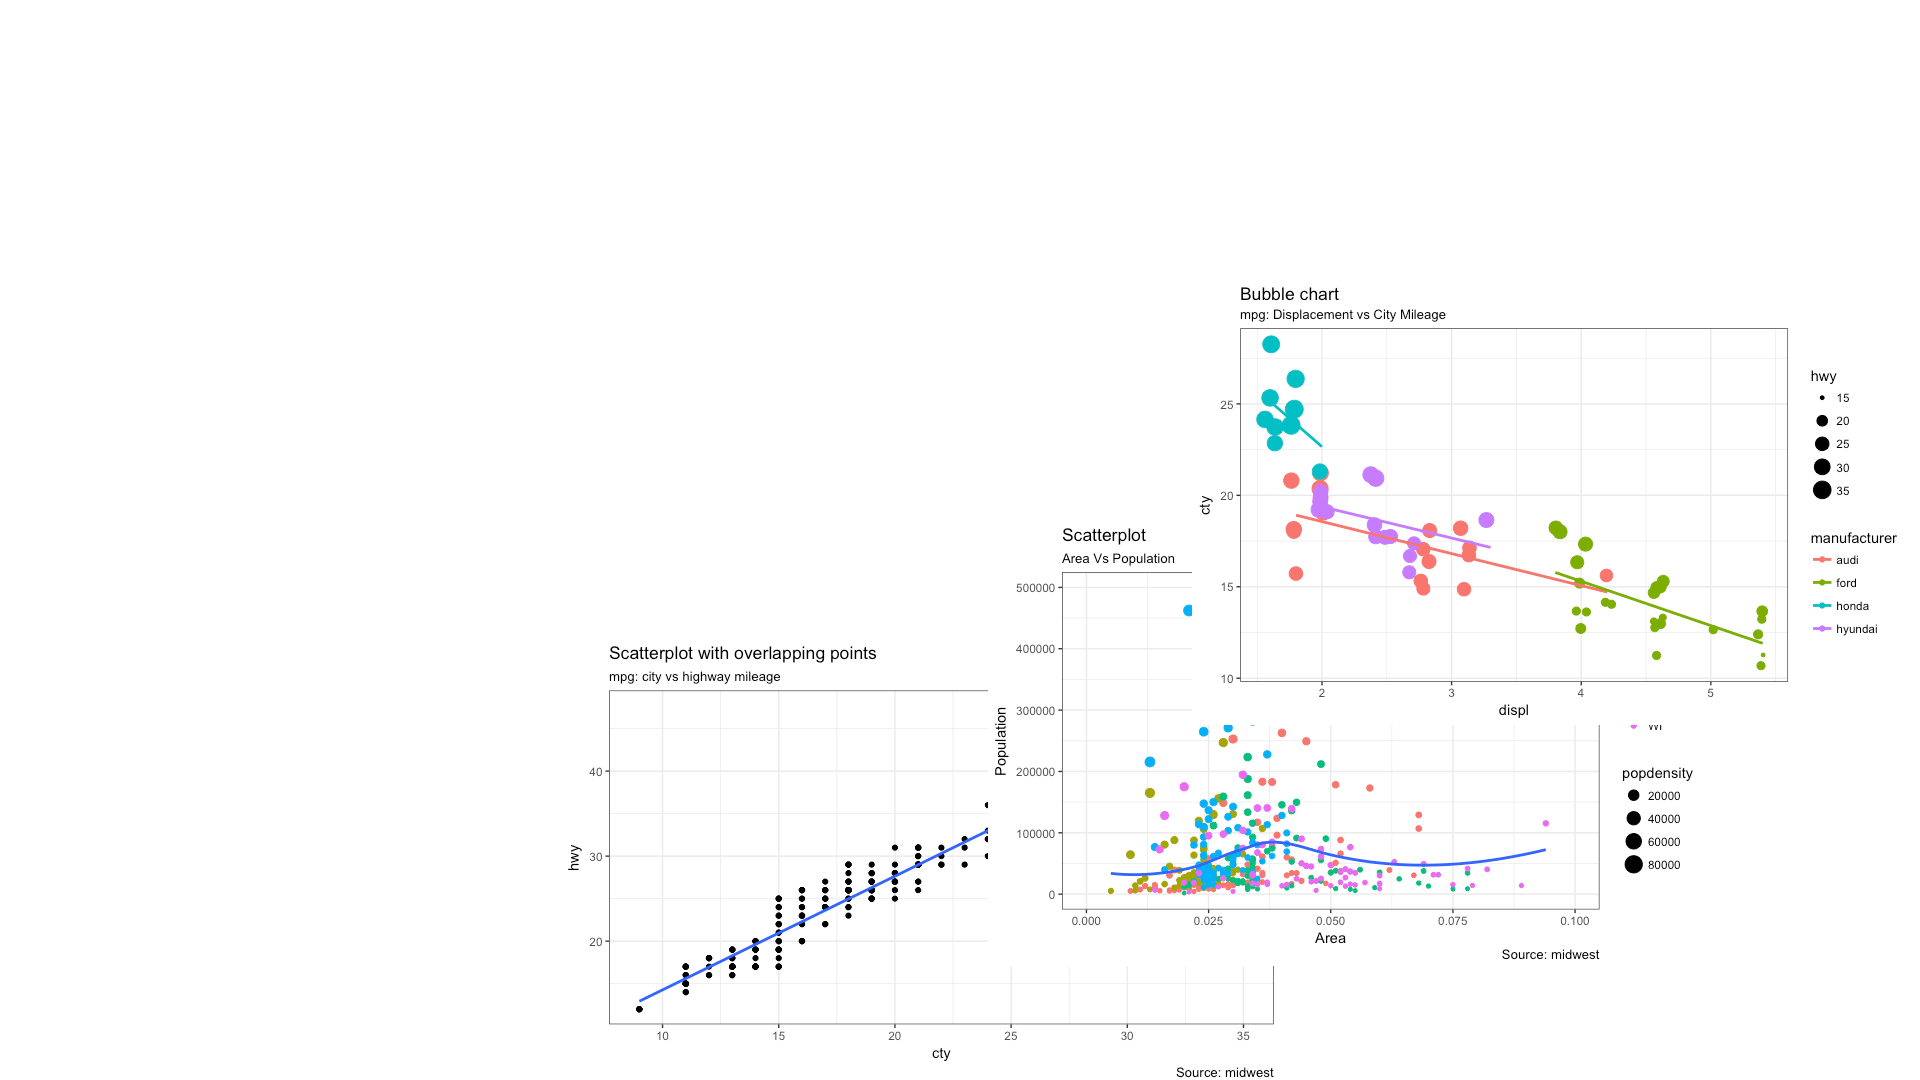
\includegraphics[width=16.5 cm]{../../Backgrounds/bg1.png}}
\usebackgroundtemplate{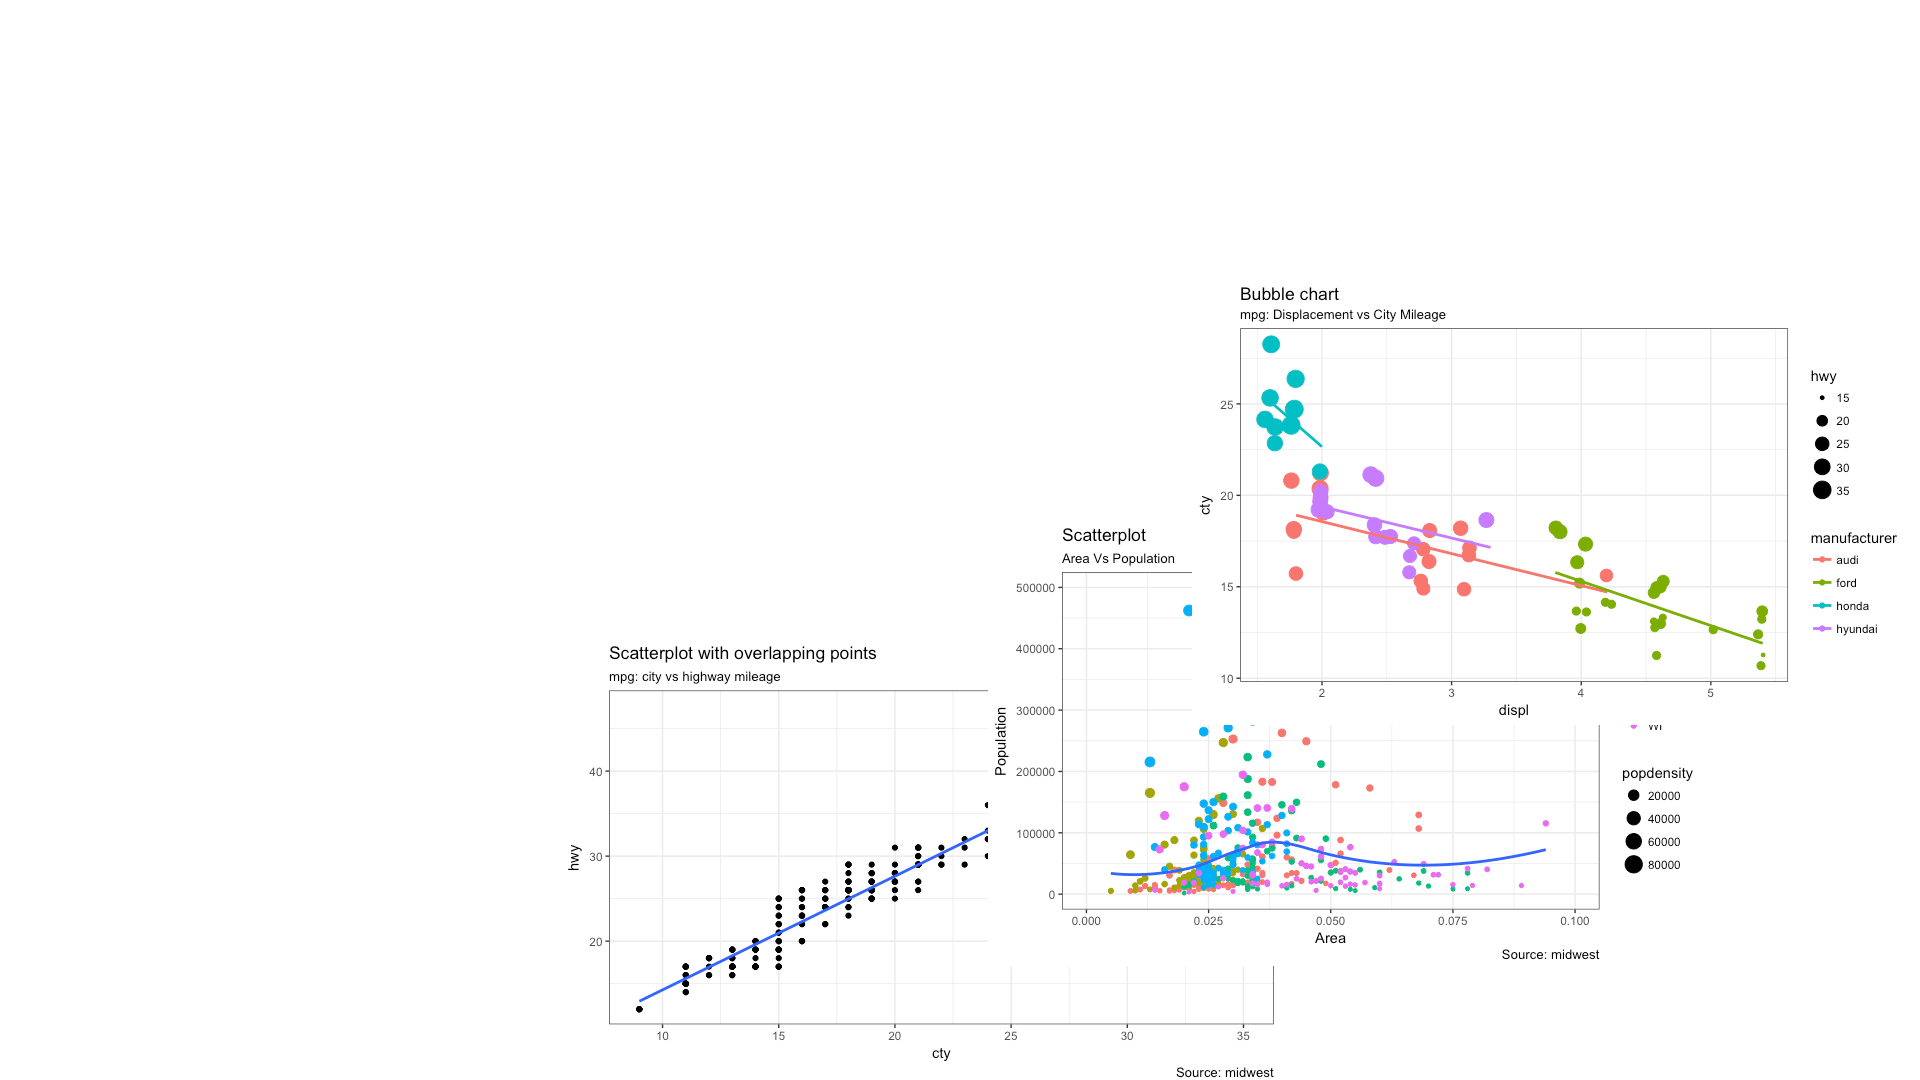
\includegraphics[width=\paperwidth]{../../Backgrounds/bg1.png}}
\setbeamercolor{background canvas}{bg=white}

\frame[plain]{\titlepage}
\setbeamertemplate{background canvas}[default]
%\usebackgroundtemplate{plain}
\section{Struktur \& Zielsetzung}
\begin{frame}[t]  
  \begin{minipage}[t]{0.45\textwidth}
    \textbf{\large{Zielsetzung:}}
    \begin{itemize}
      \item Wiederholung: 
      \begin{itemize}
        \item Arbeiten mit Datensätzen, Einlesen, Operationen in R
        \item Skalenniveaus, Variablenarten, Datentypen
      \end{itemize}
      \item Regressionen:
      \begin{itemize}
        \item Grundlagen
        \item Formen
        \item Anwendung
        \item Auswertung
        \item Darstellung
      \end{itemize}
      \item Zusammenfassung \& weiterführende Beispiele
    \end{itemize}
  \end{minipage}
  \begin{minipage}{0.45\textwidth}

  \end{minipage}
\end{frame}

\begin{frame}[t]  
  \begin{minipage}[t]{0.45\textwidth}
    \textbf{\large{Zielsetzung:}}
    \begin{itemize}
      \item Wiederholung: 
      \begin{itemize}
        \item Arbeiten mit Datensätzen, Einlesen, Operationen in R
        \item Skalenniveaus, Variablenarten, Datentypen
      \end{itemize}
      \item Regressionen:
      \begin{itemize}
        \item Grundlagen
        \item Formen
        \item Anwendung
        \item Auswertung
        \item Darstellung
      \end{itemize}
      \item Zusammenfassung \& weiterführende Beispiele
    \end{itemize}
  \end{minipage}%
  \begin{minipage}[t]{0.45\textwidth}
    \textbf{\large{Struktur:}}
    \begin{enumerate}
      \item Beispiel
      \item Theorie
      \item Praxis
      \item Take Home Message
    \end{enumerate}
    \vspace{4em}
    \begin{itemize}
      \item Daten:
      \small
      \item[] \oarrow \url{https://github.com/MKernt/Lehrprobe/tree/master/Lehrprobe}  
    \end{itemize}
  \end{minipage}
\end{frame}

%------------------
\section{Beispiel}
%------------------
\setbeamertemplate{background canvas}[default]
\setbeamercolor{background canvas}{bg=PN3}
\thispagestyle{empty}
\begin{frame} 
\begin{center}
\textcolor{SS2}{\huge{\textbf{Beispiel}}}
\end{center}
\end{frame}

\setbeamercolor{background canvas}{bg=}
\begin{frame}[t]
  \begin{minipage}[t]{0.5\textwidth}
    \begin{itemize}
        \item[] \textbf{Forschungsfrage:}
        \item Welchen Einfluss haben Bildung und Frauenrechte auf Geburtenraten?
    \end{itemize}
  \end{minipage}%
  \begin{minipage}[t]{0.5\textwidth}
    \begin{itemize}
      \item[]  
    \end{itemize}
  \end{minipage}
\end{frame}

\begin{frame}[t]
  \begin{minipage}[t]{0.5\textwidth}
    \begin{itemize}
        \item[] \textbf{Forschungsfrage:}
        \item Welchen Einfluss haben Bildung und Frauenrechte auf Geburtenraten?
        \scriptsize
        \item[] \fullcite{Jejeebhoy1995}
        \item[] \fullcite{Sagalova2021} 
        \item[] \fullcite{Samari2019}
        \item[] \fullcite{Keller2018}
    \end{itemize}
  \end{minipage}%
  \begin{minipage}[t]{0.5\textwidth}
    \begin{itemize}
      \item[] 
    \end{itemize}
  \end{minipage}
\end{frame}

\begin{frame}[t]
  \begin{minipage}[t]{0.5\textwidth}
    \begin{itemize}
      \item[] \textbf{Forschungsfrage:}
      \item Welchen Einfluss haben Bildung und Frauenrechte auf Geburtenraten?
      \scriptsize
      \item[] \fullcite{Jejeebhoy1995}
      \item[] \fullcite{Sagalova2021} 
      \item[] \fullcite{Samari2019}
      \item[] \fullcite{Keller2018}
  \end{itemize}
  \end{minipage}%
  \begin{minipage}[t]{0.5\textwidth}
    \begin{itemize}
      \item[] \textbf{Hypothesen:}
      \item[] \textbf{H1:} Je länger die obligatorische Bildung in einem Land dauert, desto niedriger ist die Geburtenrate
      \item[] \textbf{H2:} Je weniger Frauenrechte in einem Land, desto höher die Geburtenrate
      \item[] 
      \item[] \oarrow Interesse daran inwiefern die Daten miteinander korrelieren
    \end{itemize}
  \end{minipage}
\end{frame}

\begin{frame}[t]
  \begin{minipage}[t]{0.5\textwidth}
    \begin{itemize}
      \item[] \textbf{Forschungsfrage:}
      \item Welchen Einfluss haben Bildung und Frauenrechte auf Geburtenraten?
      \scriptsize
      \item[] \fullcite{Jejeebhoy1995}
      \item[] \fullcite{Sagalova2021} 
      \item[] \fullcite{Samari2019}
      \item[] \fullcite{Keller2018}
  \end{itemize}
  \end{minipage}%
  \begin{minipage}[t]{0.5\textwidth}
    \begin{itemize}
      \item[] \textbf{Hypothesen:}
      \item[] \textbf{H1:} Je länger die obligatorische Bildung in einem Land dauert, desto niedriger ist die Geburtenrate
      \item[] \textbf{H2:} Je weniger Frauenrechte in einem Land, desto höher die Geburtenrate
      \item[] 
      \item[] \oarrow Interesse daran inwiefern die Daten miteinander korrelieren
      \item[] \footnotesize \begin{tcolorbox}[title=Achtung!, colframe=red!80!black, colback=orange!25]
        \centering
        Korrelation $\neq$ Kausalbeziehung
      \end{tcolorbox}
    \end{itemize}
  \end{minipage}
\end{frame}

\begin{frame}[t]
  \begin{minipage}[t]{0.5\textwidth}
    \begin{itemize}
        \item[] \textbf{Datensatz}
        \item Basierend auf:
        \begin{itemize}
          \item UN Daten
          \item[] \oarrow \url{http://data.un.org/} 
          \item CIRI Human Rights Dataset 
          \item[] \oarrow \url{http://www.humanrightsdata.com/p/data-documentation.html}
        \end{itemize}
        \item Querschnittsdaten
    \end{itemize}
  \end{minipage}%
  \begin{minipage}[t]{0.5\textwidth}
    \begin{itemize}
      \item[]
    \end{itemize}
  \end{minipage}
\end{frame}

    \begin{frame}[t]
      \begin{minipage}[t]{0.5\textwidth}
        \vspace{-2.5em}
        \begin{itemize}
            \item[] \textbf{Datensatz}
            \item Basierend auf:
            \begin{itemize}
              \item UN Daten
              \item[] \oarrow \url{http://data.un.org/} 
              \item CIRI Human Rights Dataset 
              \item[] \oarrow \url{http://www.humanrightsdata.com/p/data-documentation.html}
            \end{itemize}
            \item Querschnittsdaten
        \end{itemize}
      \end{minipage}%
      \begin{minipage}[t]{0.5\textwidth}
        \centering
        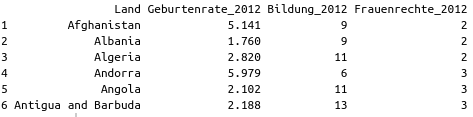
\includegraphics[scale=0.4]{../Plots/data_head.png}
        \begin{itemize}
          \item Land
          \item Geburtenrate
          \item Durchschnittliche Bildungsdauer (in Jahren)
          \item Frauenrechte
          \item[] \oarrow 0: keine Rechte im Gesetz; 3: (alle) Rechte im Gesetz und in der Praxis
        \end{itemize}
      \end{minipage}
    \end{frame}

%------------------
\section{Theorie}
%------------------
\setbeamertemplate{background canvas}[default]
\setbeamercolor{background canvas}{bg=PN3}
\thispagestyle{empty}
\begin{frame} 
\begin{center}
\textcolor{SS2}{\huge{\textbf{Theorie}}}
\end{center}
\end{frame}

\setbeamercolor{background canvas}{bg=}
  \subsection{Grundlagen}
    \begin{frame}[t]
      \textbf{Wozu Regressionsanalyse?}
      \begin{minipage}[t]{0.5\textwidth}
        \begin{itemize}
            \item Einfluss einer oder mehrerer unabhängiger Variablen auf (\textbf{x}) \linebreak \textbf{eine} abhängige Variable (\textbf{y})
            \item[] \oarrow Regression von Y auf X
        \end{itemize}
      \end{minipage}%
      \begin{minipage}[t]{0.5\textwidth}
        \begin{itemize}
          \item[] 
        \end{itemize}
      \end{minipage}
    \end{frame}

    \begin{frame}[t]
      \textbf{Wozu Regressionsanalyse?}
      \begin{minipage}[t]{0.45\textwidth}
        \vspace{-11.5em}
        \begin{itemize}
            \item Einfluss einer oder mehrerer unabhängiger Variablen auf (\textbf{x}) \linebreak \textbf{eine} abhängige Variable (\textbf{y})\item[] \oarrow Regression von Y auf X
            \item Formel: $y = a + bx$
            \begin{itemize}
              \item a = Schnittpunkt y-Achse (intercept)
              \item b = Steigung (slope)
            \end{itemize}
        \end{itemize}
      \end{minipage}%
      \begin{minipage}[t]{0.45\textwidth}
        %\begin{figure}
        %\vspace{-5.5}
        \centering
        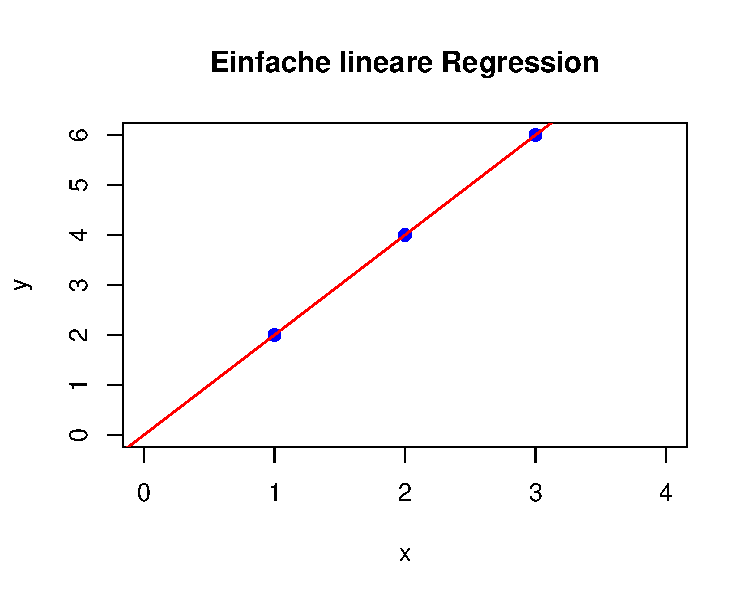
\includegraphics[scale=0.5]{../Plots/reg_lin_1.pdf}
        \begin{table}[]
          \begin{tabular}{lllll}
          \multicolumn{1}{l|}{\textbf{$x_i$}} & 1 & 2 & 3 &  \\ \cline{1-4}
          \multicolumn{1}{l|}{$y_i$} & 2 & 4 & 6 &  \\
                                 &   &   &   &  \\
                                 &   &   &   & 
          \end{tabular}
          \end{table}
        %\end{figure}
      \end{minipage}
    \end{frame}

    \begin{frame}[t]
      \textbf{Wozu Regressionsanalyse?}
      \begin{minipage}[t]{0.45\textwidth}
        \vspace{-11.5em}
        \begin{itemize}
            \item Einfluss einer oder mehrerer unabhängiger Variablen auf (\textbf{x}) \linebreak \textbf{eine} abhängige Variable (\textbf{y})\item[] \oarrow Regression von Y auf X
        \end{itemize}
      \end{minipage}%
      \begin{minipage}[t]{0.45\textwidth}
        %\begin{figure}
        %\vspace{-5.5}
        \centering
        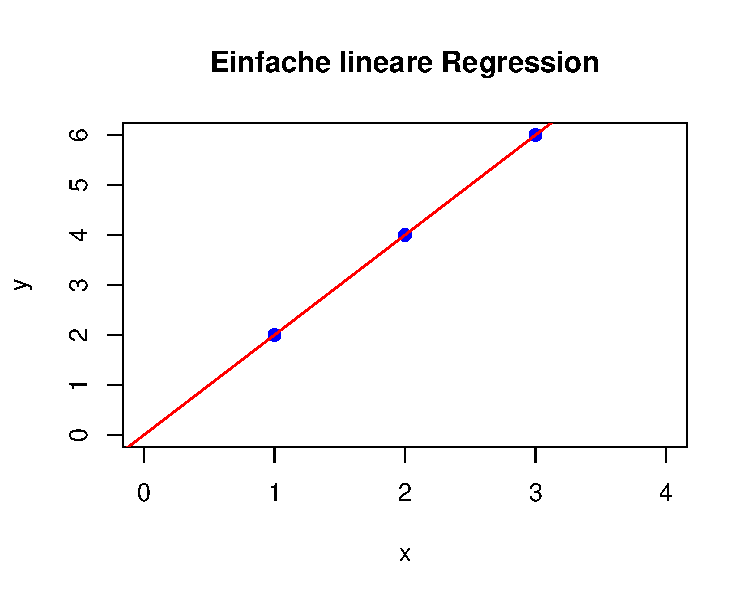
\includegraphics[scale=0.5]{../Plots/reg_lin_1.pdf}
        \begin{table}[]
          \begin{tabular}{lllll}
          \multicolumn{1}{l|}{\textbf{$x_i$}} & 1 & 2 & 3 &  \\ \cline{1-4}
          \multicolumn{1}{l|}{$y_i$} & 2 & 4 & 6 &  \\
                                 &   &   &   &  \\
                                 &   &   &   & 
          \end{tabular}
          \end{table}
        %\end{figure}
      \end{minipage}
    \end{frame}

    \begin{frame}[t]
      \begin{minipage}[t]{0.45\textwidth}
        \vspace{-11.5em}
        \begin{itemize}
          \item Zusammenhang fast nie perfekt
        \end{itemize}
    \end{minipage}%
    \begin{minipage}[t]{0.45\textwidth}
      \centering
      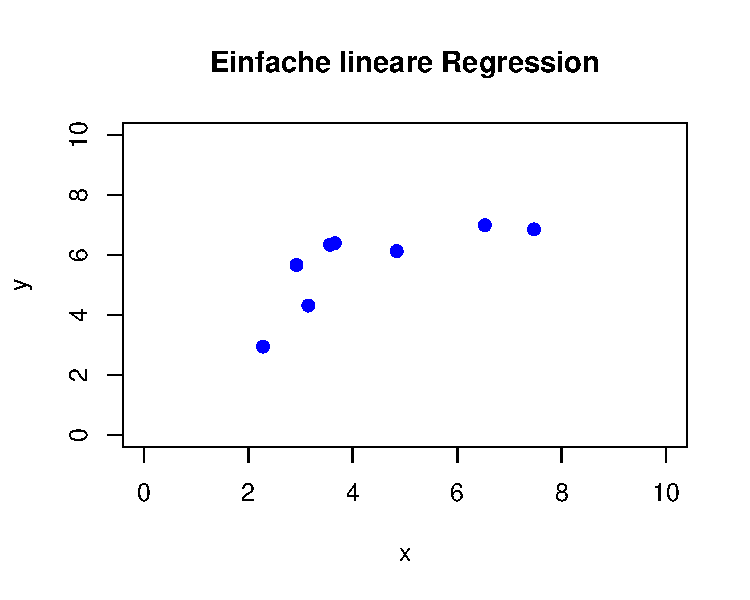
\includegraphics[scale=0.5]{../Plots/reg_lin_2.pdf}
    \end{minipage}
  \end{frame}

  \begin{frame}[t]
    \begin{minipage}[t]{0.45\textwidth}
      \vspace{-11.5em}
      \begin{itemize}
        \item Zusammenhang fast nie perfekt
      \end{itemize}
  \end{minipage}%
  \begin{minipage}[t]{0.45\textwidth}
    \centering
    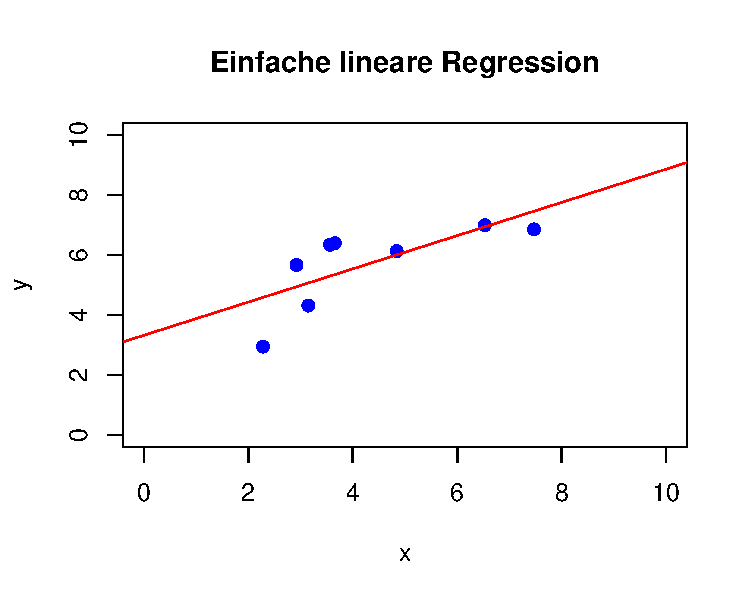
\includegraphics[scale=0.5]{../Plots/reg_lin_3.pdf}
  \end{minipage}
\end{frame}

\begin{frame}[t]
  \begin{minipage}[t]{0.45\textwidth}
    \vspace{-11.5em}
    \begin{itemize}
      \item Zusammenhang fast nie perfekt
      \item Hinzufügen eines Fehlerterms
      \item[] \oarrow $y = a + b * x + \epsilon_i$
      \item Konstanten (Koeffizienten):  
      \begin{itemize}
        \item $a$ = Schnittpunkt y-Achse (intercept)
        \item $b$ = Steigung (slope) 
      \end{itemize}
      \item Tatsächliche Werte der Punkte
      \begin{itemize}
        \item $x$ = unabhängige Variable
        \item $y$ = abhängige Variable
      \end{itemize} 
      \item Fehlerterm (Residuen)
      \begin{itemize}
        \item $\epsilon$ = Abweichung der Punkte von der Ideallinie
      \end{itemize} 
    \end{itemize}
\end{minipage}%
\begin{minipage}[t]{0.45\textwidth}
  \centering
  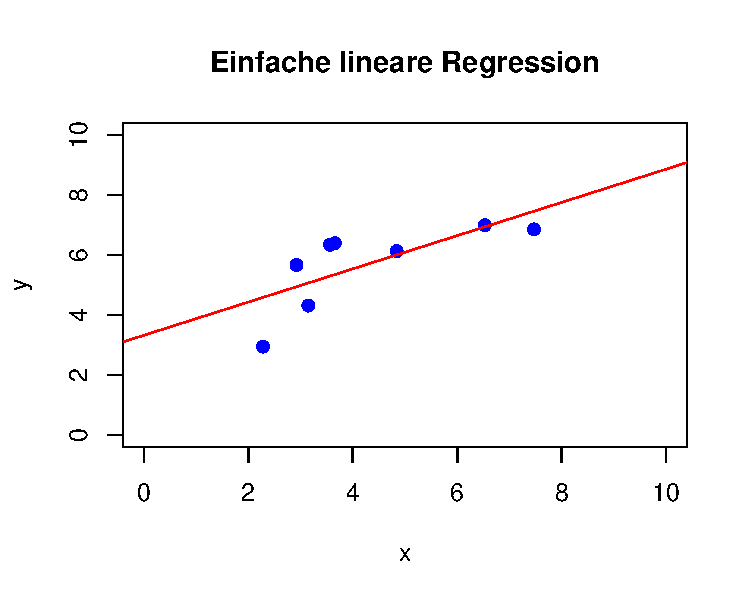
\includegraphics[scale=0.5]{../Plots/reg_lin_3.pdf}
\end{minipage}
\end{frame}

\begin{frame}[t]
  \begin{minipage}[t]{0.45\textwidth}
    \vspace{-11.5em}
    \begin{itemize}
      \item Zusammenhang fast nie perfekt
      \item Hinzufügen eines Fehlerterms
      \item[] \oarrow $y = a + b * x + \epsilon$
      \item Konstanten (Koeffizienten):  
      \begin{itemize}
        \item $a$ = Schnittpunkt y-Achse (intercept)
        \item $b$ = Steigung (slope) 
      \end{itemize}
      \item Tatsächliche Werte der Punkte
      \begin{itemize}
        \item $x$ = unabhängige Variable
        \item $y$ = abhängige Variable
      \end{itemize} 
      \item Fehlerterm
      \begin{itemize}
        \item $\epsilon$ = Zufällige Fehler/Rauschen
      \end{itemize} 
    \end{itemize}
\end{minipage}%
\begin{minipage}[t]{0.45\textwidth}
  \centering
  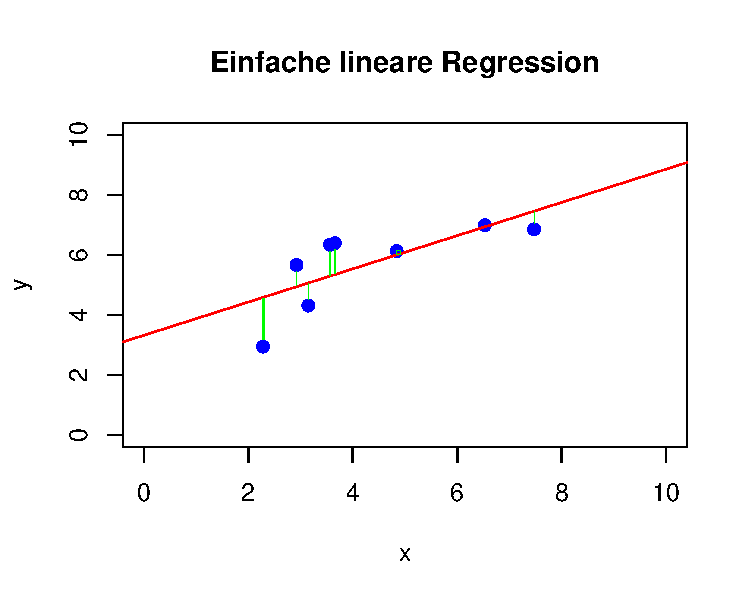
\includegraphics[scale=0.5]{../Plots/reg_lin_4.pdf}
\end{minipage}
\end{frame}

\begin{frame}[t]
  \begin{minipage}[t]{0.45\textwidth}
    \vspace{-11.5em}
    \begin{itemize}
      \item Residuen sind die \textbf{Abweichungen} der \textbf{geschätzten y-Werte} zu den \textbf{tatsächlichen y-Werten} 
      \item Ziel ist es die Residuen möglichst klein zu halten
      \item[] \oarrow Verfahren: Ordinary Least Squares (OLS)
    \end{itemize}
\end{minipage}%
\begin{minipage}[t]{0.45\textwidth}
  \centering
  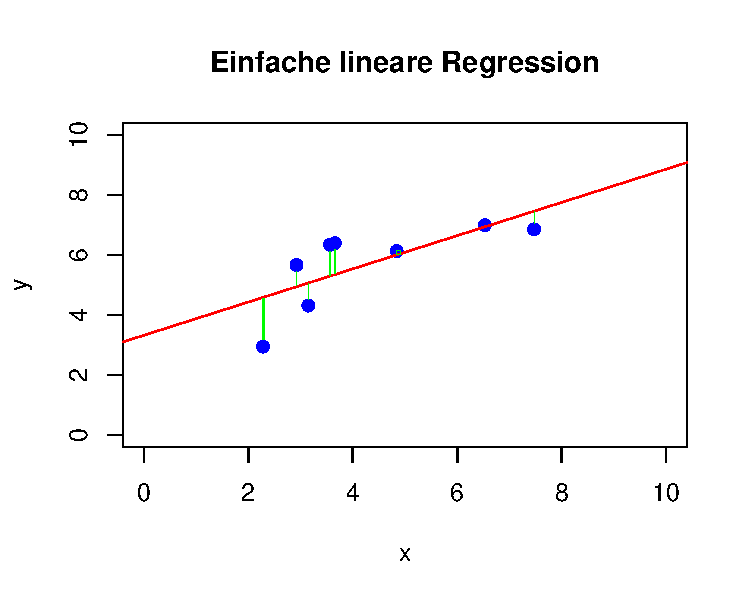
\includegraphics[scale=0.5]{../Plots/reg_lin_4.pdf}
\end{minipage}
\end{frame}

\begin{frame}[t]
  \begin{minipage}[t]{0.45\textwidth}
    \vspace{-11.5em}
    \begin{itemize}
      \item Residuen sind die \textbf{Abweichungen} der \textbf{geschätzten y-Werte} zu den \textbf{tatsächlichen y-Werten} 
      \item Ziel ist es die Residuen möglichst klein zu halten
      \item[] \oarrow Verfahren: Ordinary Least Squares (OLS)
    \end{itemize}
\end{minipage}%
\begin{minipage}[t]{0.45\textwidth}
  \centering
  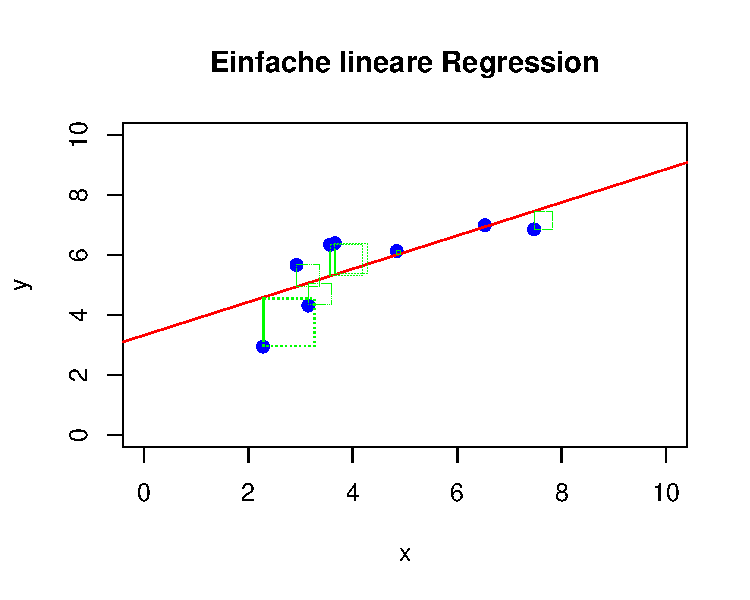
\includegraphics[scale=0.5]{../Plots/reg_lin_5.pdf}
\end{minipage}
\end{frame}

\begin{frame}[t]
  \begin{minipage}[t]{0.45\textwidth}
    \vspace{-11.5em}
    \begin{itemize}
      \item Residuen sind die \textbf{Abweichungen} der \textbf{geschätzten y-Werte} zu den \textbf{tatsächlichen y-Werten} 
      \item Ziel ist es die Residuen möglichst klein zu halten
      \item[] \oarrow Verfahren: Ordinary Least Squares (OLS)
    \end{itemize}
\end{minipage}%
\begin{minipage}[t]{0.45\textwidth}
  \begin{center}
    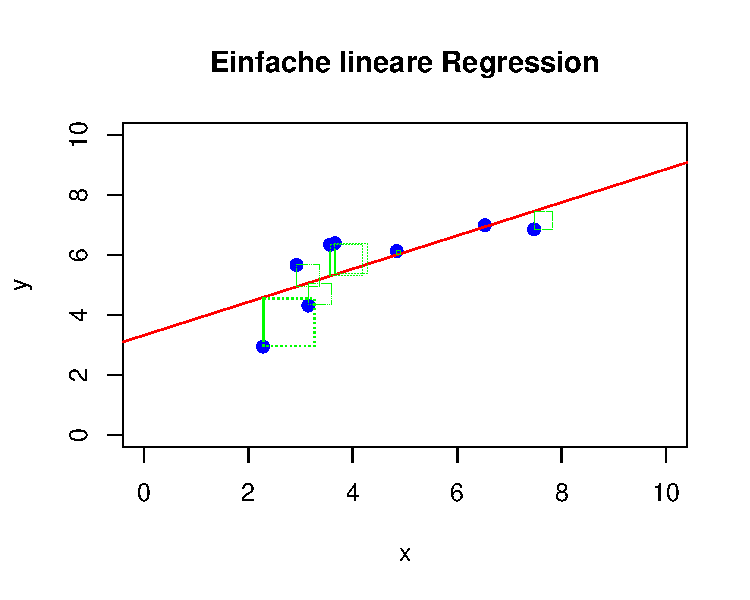
\includegraphics[scale=0.5]{../Plots/reg_lin_5.pdf}
  \end{center}

  \vspace{-1em}
  \footnotesize
  \hspace{2em} $b = \frac{\sum_{i = 1}^{n}(x_i-\bar{x})*(y_i-\bar{y})}{\sum_{i = 1}^{n}(x_i-\bar{x})^2} $ 

  \medskip
  \hspace{2em} $a = \bar{y} - b * \bar{x}$

  \medskip
  \hspace{2em} $\bar{x}$ und $\bar{y} = $  Mittelwerte aller x und y

  \end{minipage}
\end{frame}


  \subsection{Formen}
    \begin{frame}[t]
      \begin{minipage}{0.45\textwidth}
        \vspace{1em}
        \begin{enumerate}
          \item \textbf{Lineare Regression}
          \item Multiple lineare Regression
          \item Logistische Regression
          \item ...
        \end{enumerate}
    \end{minipage}%
    \begin{minipage}[t]{0.45\textwidth}
      \begin{tcolorbox}
        \begin{center}
          $y = a + b * x + \epsilon$
        \end{center}
      \end{tcolorbox}
      \begin{itemize}
        \item[] \textbf{Merkmale:}
        \begin{itemize} 
          \item Linearität zwischen x und Mittelwert von y
          \item Kontinuierliche abhängige Variable
        \end{itemize}
        \item[] \textbf{Annahmen:}
        \begin{itemize} 
          \footnotesize
          \item Der Erwartungswert der Residuen ist Null 
          \item Die Fehlerterme sind unkorreliert
          \item Es herrscht Homoskedastizität
          \item Die Fehlerterme sind normalverteilt
        \end{itemize}
      \end{itemize}
    \end{minipage}
    \end{frame}

    \begin{frame}[t]
      \begin{minipage}{0.45\textwidth}
        %\vspace{-11.5em}
        \begin{enumerate}
          \item Lineare Regression
          \item \textbf{Multiple lineare Regression}
          \item Logistische Regression
          \item ...
        \end{enumerate}
    \end{minipage}%
    \begin{minipage}[t]{0.45\textwidth}
      \begin{tcolorbox}
        \begin{center}
          $y_i = a + b_1 * x_{i1} + b_2 * x_{i2} + ... + \epsilon_i$, $i = 1, ..., n$
          \end{center}
        \end{tcolorbox}
      \begin{itemize}
        \item[] \textbf{Merkmale:}
        \item Siehe einfache lineare Regression
        \item Mehrere unabhängige Variablen
        \item Unabhängige Variablen müssen nicht kontinuierlich sein
      \end{itemize}
    \end{minipage}
    \end{frame}

    \begin{frame}[t]
      \begin{minipage}{0.45\textwidth}
        %\vspace{-11.5em}
        \begin{enumerate}
          \item Lineare Regression
          \item \textbf{Multiple lineare Regression}
          \item Logistische Regression
          \item ...
        \end{enumerate}
    \end{minipage}%
    \begin{minipage}[t]{0.45\textwidth}
      \begin{tcolorbox}
        \begin{center}
          $y_i = a + b_1 * x_{i1} + b_2 * x_{i2} + ... + \epsilon_i$, $i = 1, ..., n$
          \end{center}
        \end{tcolorbox}
      \begin{itemize}
        \item[] \textbf{Merkmale:}
        \item Siehe einfache lineare Regression
        \item Mehrere unabhängige Variablen
        \item Unabhängige Variablen müssen nicht kontinuierlich sein
      \end{itemize}
      \begin{tcolorbox}[title=Achtung!, colframe=red!80!black, colback=orange!25]
        \centering
        Multiple $\neq$ Multivariate
      \end{tcolorbox}
    \end{minipage}
    \end{frame}

    \begin{frame}[t]
      \begin{minipage}{0.45\textwidth}
        \vspace{1em}
        \begin{enumerate}
          \item Lineare Regression
          \item Multivariate Regression
          \item \textbf{Logistische Regression}
          \item ...
        \end{enumerate}
    \end{minipage}%
    \begin{minipage}[t]{0.45\textwidth}
      \begin{tcolorbox}
        \begin{center}
          $\pi_i = \frac{1}{1+\mathrm{e}^{x_i \beta}} $
        \end{center}
      \end{tcolorbox}
      \begin{itemize}
        \item[] \textbf{Merkmale:}
        \item Dichotome abhängige Variable
        \item[] \oarrow Mann/Frau, ja/nein, etc.
      \end{itemize}
      \centering
%      \vspace{-3em}
      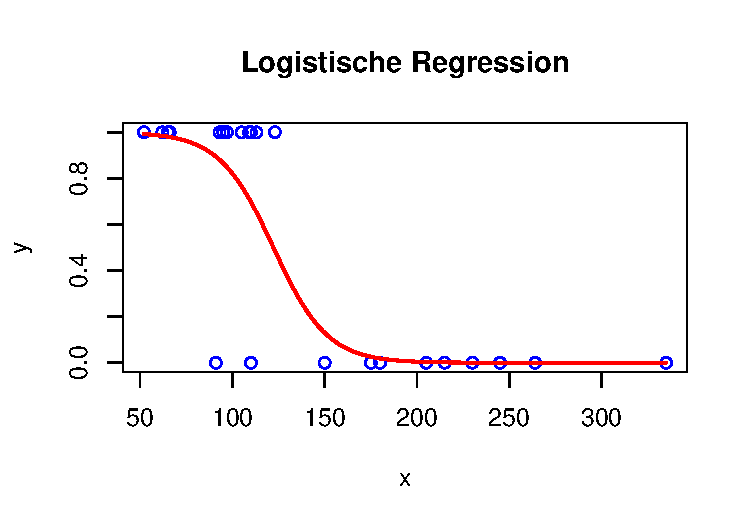
\includegraphics[scale=0.5]{../Plots/log_lin_1.pdf}
    \end{minipage}
    \end{frame}

    \begin{frame}[t]
      \begin{minipage}[t]{0.45\textwidth}
        %\vspace{-11.5em}
        \begin{enumerate}
          \item Lineare Regression
          \item Multivariate Regression
          \item Logistische Regression
          \item \textbf{...}
        \end{enumerate}
    \end{minipage}%
    \begin{minipage}[t]{0.45\textwidth}
      \begin{itemize}
        \item Ordinale Regression
        \begin{itemize}
          \item[\oarrow] AV mit mehr als zwei Kategorien (bspw. Antwortmöglichkeiten bei Umfragen)
        \end{itemize}
        \item Poisson Regression
        \begin{itemize}
          \item[\oarrow] AV mit Zählvariablen (bspw. Anzahl Anrufe bei einer Notfallnummer)
        \end{itemize}
        \item ...
      \end{itemize}
    \end{minipage}
    \end{frame}
  
%------------------
\section{Praxis}
%------------------
\setbeamertemplate{background canvas}[default]
\setbeamercolor{background canvas}{bg=PN3}
\thispagestyle{empty}
\begin{frame} 
\begin{center}
\textcolor{SS2}{\huge{\textbf{Praxis}}}
\end{center}
\end{frame}

\setbeamercolor{background canvas}{bg=}
  \subsection{Initiale Schritte}
    \begin{frame}[t, fragile]
      \begin{minipage}[t]{0.45\textwidth}
          \begin{enumerate}
              \item[] \textbf{Vorbereitung:}
              \item Datensatz herunterladen
              \item Jupyter Hub oder lokales RStudio öffnen 
              \item[] \oarrow \url{https://jupyterhub.wolke.uni-greifswald.de/}
              \item Datensatz einlesen
              \begin{itemize}
                \item via GUI, oder
                \item direkt im Script
              \end{itemize}
          \end{enumerate}
            \begin{lstlisting}
      world_data <- read.csv("world_data.csv",
        stringsAsFactors=FALSE)
            \end{lstlisting}
        \end{minipage}
        \begin{minipage}[t]{0.45\textwidth}
          \begin{enumerate}
            \item[] 
          \end{enumerate}
        \end{minipage}
    \end{frame}

    \begin{frame}[t, fragile]
      \begin{minipage}[t]{0.45\textwidth}
          \begin{enumerate}
              \item[] \textbf{Vorbereitung:}
              \item Datensatz herunterladen
              \item Jupyter Hub oder lokales RStudio öffnen 
              \item[] \oarrow \url{https://jupyterhub.wolke.uni-greifswald.de/}
              \item Datensatz einlesen
              \begin{itemize}
                \item via GUI, oder
                \item direkt im Script
              \end{itemize}
          \end{enumerate}
            \begin{lstlisting}
      world_data <- read.csv("world_data.csv",
        stringsAsFactors=FALSE)
            \end{lstlisting}
        \end{minipage}
        \begin{minipage}[t]{0.45\textwidth}
          \begin{itemize}[<+(-1)->]
            \item[] \textbf{Vorgehen:} 
            \item Erstes Sichten der Daten
            \item[] \begin{lstlisting}
head(world_data)
str(world_data)
summary(world_data)
            \end{lstlisting}
            \item Daten formatieren
            \item[] \begin{lstlisting}
world_data$Frauenrechte_2012 = as.factor
  (world_data$Frauenrechte_2012)
            \end{lstlisting}
          \end{itemize}
        \end{minipage}
    \end{frame}

  \subsection{Anwendung -- Hypothese 1}
  \begin{frame}[t, fragile]
    \begin{minipage}[t]{0.45\textwidth}
        \begin{itemize}
            \item[] \textbf{H1:} Je länger die obligatorische Bildung in einem Land dauert, desto niedriger ist die Geburtenrate
          \end{itemize}
\begin{lstlisting}
model_H1 = lm(Geburtenrate_2012 ~ Bildung_2012, 
  data=world_data)
summary(model_H1)
\end{lstlisting} 
      \end{minipage}
      \begin{minipage}[t]{0.45\textwidth}
        \begin{itemize}
          \item[]
        \end{itemize}
      \end{minipage}
  \end{frame}

  \begin{frame}[t, fragile]
    \begin{minipage}[t]{0.45\textwidth}
        \begin{itemize}
            \item[] \textbf{H1:} Je länger die obligatorische Bildung in einem Land dauert, desto niedriger ist die Geburtenrate
          \end{itemize}
\begin{lstlisting}
model_H1 = lm(Geburtenrate_2012 ~ Bildung_2012, 
  data=world_data)
summary(model_H1)
\end{lstlisting} 
      \end{minipage}
      \begin{minipage}[t]{0.45\textwidth}
        \begin{itemize}
          \item[] \textbf{Output:}
        \end{itemize}
        \begin{center}
          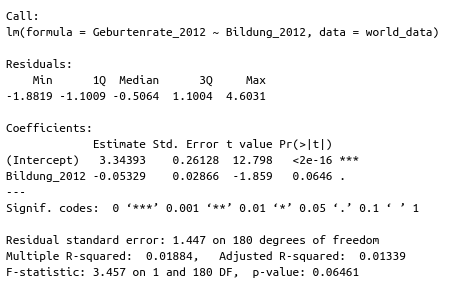
\includegraphics[scale=0.3]{../Plots/summary_H1.png}
        \end{center}
      \end{minipage}
  \end{frame}

  \begin{frame}[t, fragile]
    \begin{minipage}[t]{0.45\textwidth}
        \begin{itemize}
            \item[] \textbf{H1:} Je länger die obligatorische Bildung in einem Land dauert, desto niedriger ist die Geburtenrate
          \end{itemize}
\begin{lstlisting}
model_H1 = lm(Geburtenrate_2012 ~ Bildung_2012, 
  data=world_data)
summary(model_H1)
\end{lstlisting} 
      \end{minipage}
      \begin{minipage}[t]{0.45\textwidth}
        \begin{itemize}
          \item[] \textbf{Output:}
        \end{itemize}
        \begin{center}
          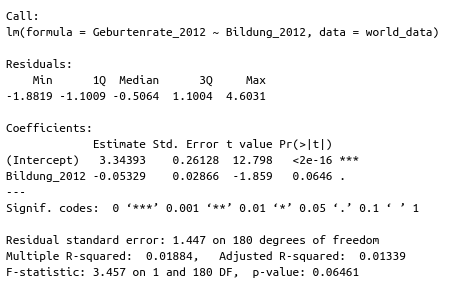
\includegraphics[scale=0.3]{../Plots/summary_H1.png}
        \end{center}
        \vspace{-1em}
        \scriptsize
        \begin{itemize}[<+(-1)->]
          \item[] \textbf{Interpretation:}
          \item Intercept  = 3.34 \oarrow bei 0 Jahren Schulzeit durchschnittlich 3.34 Kinder 
          \item Bildung 2012 = -0.05 \oarrow pro Einheit Schulbildung nimmt durchschnittlich Anzahl an Kindern um 0.05 ab (p-Wert $ >$ 0.05 \oarrow nicht signifikant)
          \item R\textsuperscript{2} = 0.018 \oarrow lediglich 1.8\% der Varianz der Daten werden durch das Modell erklärt
        \end{itemize}
      \end{minipage}
  \end{frame}


  \subsection{Darstellung -- Hypothese 1} 
  \begin{frame}[t, fragile]
    \begin{minipage}[t]{0.45\textwidth}
        \begin{itemize}
            \item[] \textbf{H1:} Je länger die obligatorische Bildung in einem Land dauert, desto niedriger ist die Geburtenrate
          \end{itemize}
\begin{lstlisting}
plot(y = world_data$Geburtenrate_2012, 
  x = world_data$Bildung_2012, 
  pch = 19, 
  col = "blue", 
  main="Plot H1", 
  xlab = "Bildung in Jahren", 
  ylab = "Geburtenrate")

abline(lm(world_data$Geburtenrate_2012 ~ 
  world_data$Bildung_2012), 
  col = "red")
\end{lstlisting} 
      \end{minipage}
      \begin{minipage}[t]{0.45\textwidth}
        \begin{itemize}
          \item[]
        \end{itemize}
      \end{minipage}
  \end{frame}

  \begin{frame}[t, fragile]
    \begin{minipage}[t]{0.45\textwidth}
        \begin{itemize}
            \item[] \textbf{H1:} Je länger die obligatorische Bildung in einem Land dauert, desto niedriger ist die Geburtenrate
          \end{itemize}
\begin{lstlisting}
plot(y = world_data$Geburtenrate_2012, 
  x = world_data$Bildung_2012, 
  pch = 19, 
  col = "blue", 
  main="Plot H1", 
  xlab = "Bildung in Jahren", 
  ylab = "Geburtenrate")

abline(lm(world_data$Geburtenrate_2012 ~ 
  world_data$Bildung_2012), 
  col = "red")
\end{lstlisting} 
      \end{minipage}
      \begin{minipage}[t]{0.45\textwidth}
        \begin{itemize}
          \item[] \textbf{Output:}
        \end{itemize}

        \begin{center}
          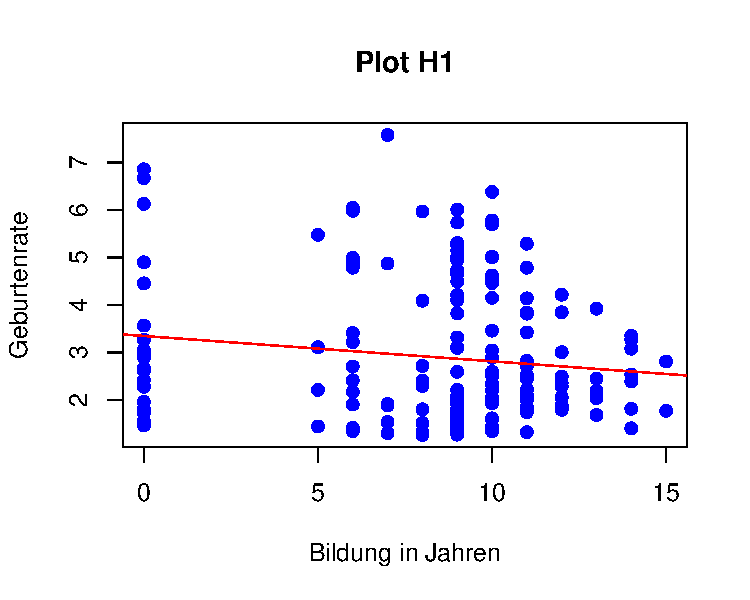
\includegraphics[scale=0.5]{../Plots/plot_H1.pdf}
        \end{center}
      \end{minipage}
  \end{frame}

\subsection{Aufgabe -- Hypothese 2}
  \begin{frame}[t, fragile]
    \begin{minipage}[t]{0.45\textwidth}
        \begin{itemize}
          \item[] \textbf{H2:} Je weniger Frauenrechte in einem Land, desto höher die Geburtenrate
          \item Führen Sie folgende Schritte aus:
          \begin{itemize}
            \item Erstellung Ergebnistabelle
            \item Interpretation der Ergebnisse
            \item Plotten der Regression
          \end{itemize}
        \end{itemize}
      \end{minipage}
      \begin{minipage}[t]{0.45\textwidth}
        \centering
        \textbf{Zeit: 10 Minuten}
      \end{minipage}
  \end{frame}

  \begin{frame}[t, fragile]
    %\vspace{-7em}
    \begin{minipage}[t]{0.45\textwidth}
        \begin{itemize}
          \item[] \textbf{H2:} Je weniger Frauenrechte in einem Land, desto höher die Geburtenrate
        \end{itemize} 
        \begin{lstlisting}
model_H2 = lm(Geburtenrate_2012 ~ 
  Frauenrechte_2012, 
  data=world_data)
summary(model_H2)

plot(y = world_data$Geburtenrate_2012, 
  x = world_data$Frauenrechte_2012, 
  pch = 19, 
  col = "blue", 
  main="Plot H1", 
  xlab = "Level Frauenrechte", 
  ylab = "Geburtenrate")          
        \end{lstlisting} 
      \end{minipage}%
      \begin{minipage}[t]{0.45\textwidth}
        \vspace{-1em}
        \centering
        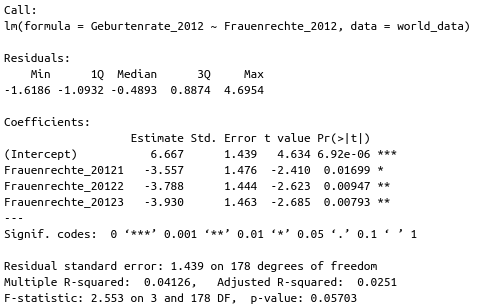
\includegraphics[scale=0.3]{../Plots/summary_H2.png}\\

        %\vspace{-1em}
        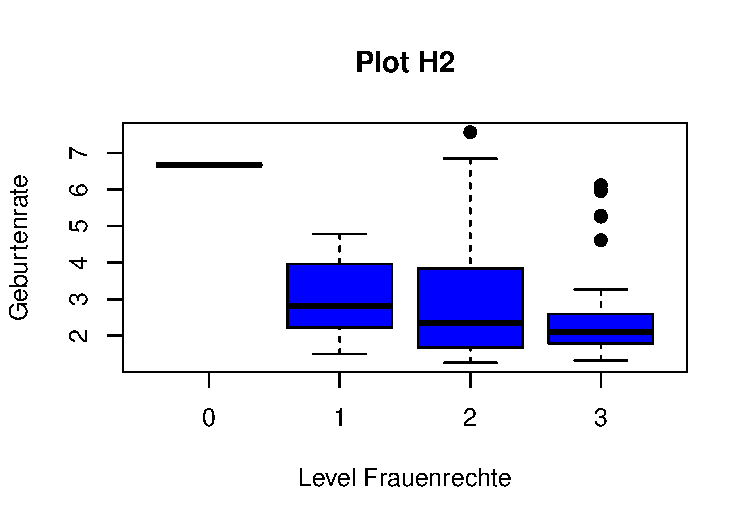
\includegraphics[scale=0.5]{../Plots/plot_H2.pdf}
      \end{minipage}
  \end{frame}


  \begin{frame}[t, fragile]
    %\vspace{-7em}
    \begin{minipage}[t]{0.5\textwidth}
        \begin{itemize}
          \item[] Was, wenn beide unabhängige Variablen ins das Modell aufgenommen werden?
        \end{itemize} 
%         \begin{lstlisting}
% model_H2 = lm(Geburtenrate_2012 ~ 
%   Frauenrechte_2012, 
%   data=world_data)
% summary(model_H2)

% plot(y = world_data$Geburtenrate_2012, 
%   x = world_data$Frauenrechte_2012, 
%   pch = 19, 
%   col = "blue", 
%   main="Plot H1", 
%   xlab = "Level Frauenrechte", 
%   ylab = "Geburtenrate")          
%         \end{lstlisting} 
      \end{minipage}%
      \begin{minipage}[t]{0.45\textwidth}
        \vspace{-1em}
        \centering
        % 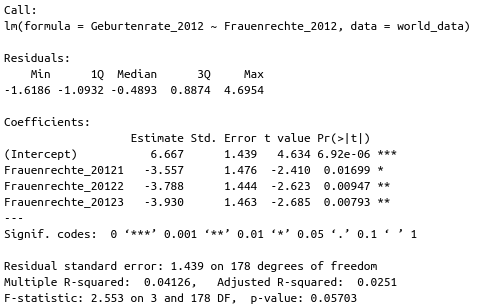
\includegraphics[scale=0.3]{../Plots/summary_H2.png}\\

        % %\vspace{-1em}
        % 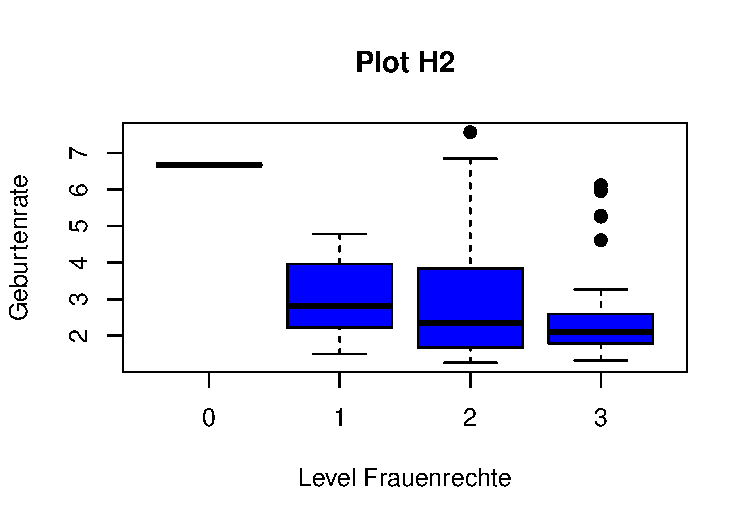
\includegraphics[scale=0.5]{../Plots/plot_H2.pdf}
      \end{minipage}
  \end{frame}

  \begin{frame}[t, fragile]
    %\vspace{-7em}
    \begin{minipage}[t]{0.45\textwidth}
        \begin{itemize}
          \item[] Was, wenn beide unabhängigen Variablen in das Modell aufgenommen werden?
        \end{itemize} 
        \begin{lstlisting}
model_multi <- lm(Geburtenrate_2012 ~ 
  Bildung_2012 + 
  Frauenrechte_2012, 
  data = world_data)        
        \end{lstlisting} 
      \end{minipage}%
      \begin{minipage}[t]{0.45\textwidth}
        \vspace{-1em}
        \centering
        % 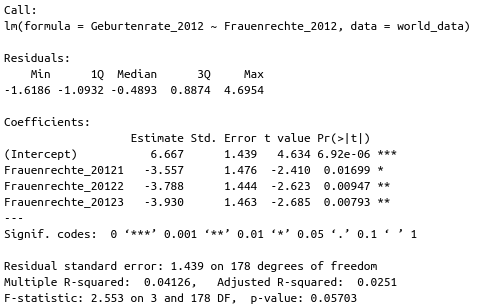
\includegraphics[scale=0.3]{../Plots/summary_H2.png}\\

        % %\vspace{-1em}
        % 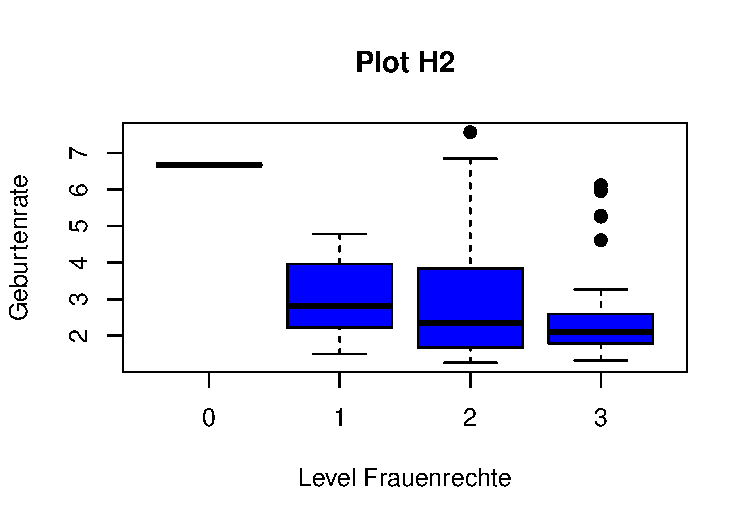
\includegraphics[scale=0.5]{../Plots/plot_H2.pdf}
      \end{minipage}
  \end{frame}

  \begin{frame}[t, fragile]
    %\vspace{-7em}
    \begin{minipage}[t]{0.45\textwidth}
        \begin{itemize}
          \item[] Was, wenn beide unabhängigen Variablen in das Modell aufgenommen werden?
        \end{itemize} 
        \begin{lstlisting}
model_multi <- lm(Geburtenrate_2012 ~ 
  Bildung_2012 + 
  Frauenrechte_2012, 
  data = world_data)        
        \end{lstlisting} 

        \centering
        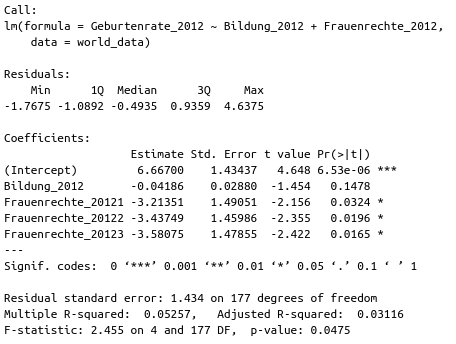
\includegraphics[scale=0.3]{../Plots/sum_multi.png}
      \end{minipage}%
      \begin{minipage}[t]{0.45\textwidth}
        \vspace{-1em}
        \centering
        % 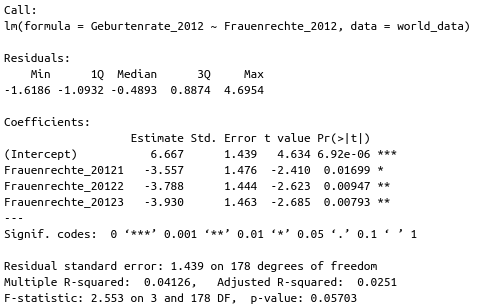
\includegraphics[scale=0.3]{../Plots/summary_H2.png}\\

        % %\vspace{-1em}
        % 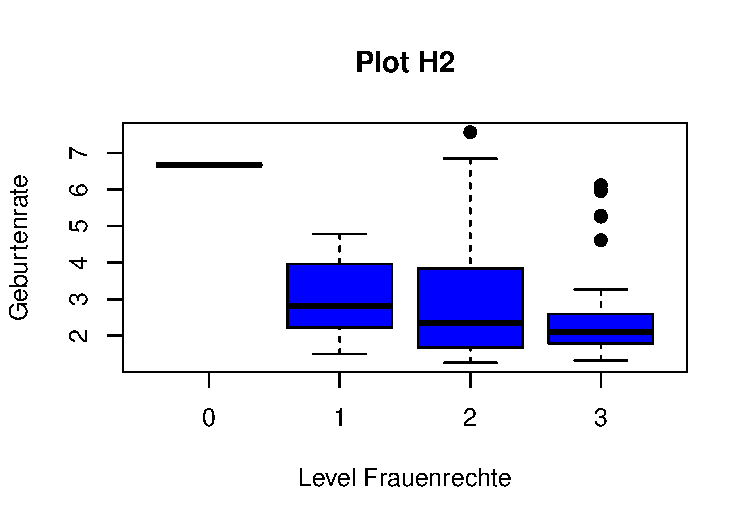
\includegraphics[scale=0.5]{../Plots/plot_H2.pdf}
      \end{minipage}
  \end{frame}

  \begin{frame}[t, fragile]
    %\vspace{-7em}
    \begin{minipage}[t]{0.45\textwidth}
        \begin{itemize}
          \item[] Was, wenn beide unabhängigen Variablen in das Modell aufgenommen werden?
        \end{itemize} 
        \begin{lstlisting}
model_multi <- lm(Geburtenrate_2012 ~ 
  Bildung_2012 + 
  Frauenrechte_2012, 
  data = world_data)        
        \end{lstlisting} 
        \centering
        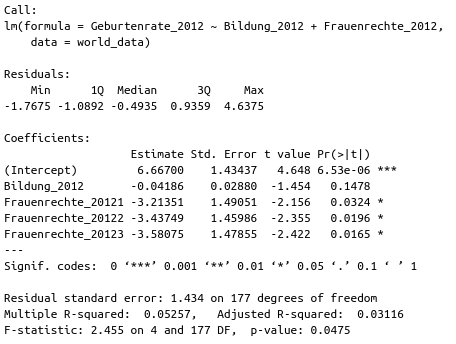
\includegraphics[scale=0.3]{../Plots/sum_multi.png}
      \end{minipage}%
      \begin{minipage}[t]{0.45\textwidth}
        \vspace{-1em}

        \centering
        \begin{lstlisting}
library(relaimpo)
calc.relimp(model_multi, type="lmg",rela=T,rank=T)    
                  \end{lstlisting} 

        % %\vspace{-1em}
        % 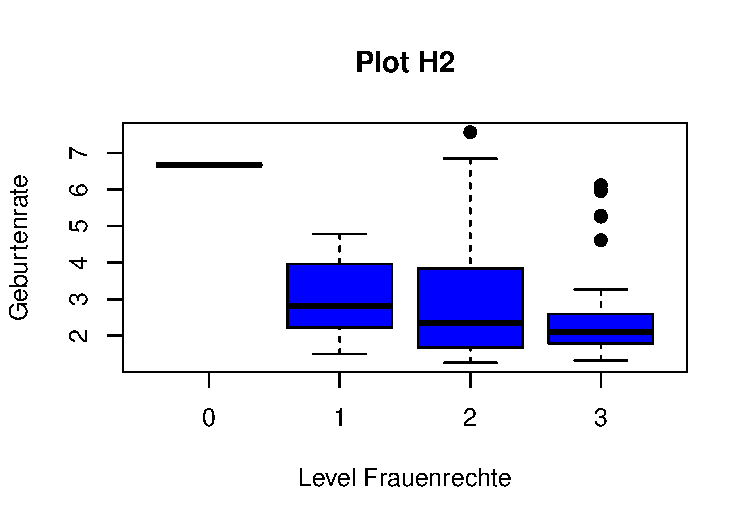
\includegraphics[scale=0.5]{../Plots/plot_H2.pdf}
      \end{minipage}
  \end{frame}

  \begin{frame}[t, fragile]
    %\vspace{-7em}
    \begin{minipage}[t]{0.45\textwidth}
        \begin{itemize}
          \item[] Was, wenn beide unabhängigen Variablen in das Modell aufgenommen werden?
        \end{itemize} 
        \begin{lstlisting}
model_multi <- lm(Geburtenrate_2012 ~ 
  Bildung_2012 + 
  Frauenrechte_2012, 
  data = world_data)        
        \end{lstlisting} 
        \centering
        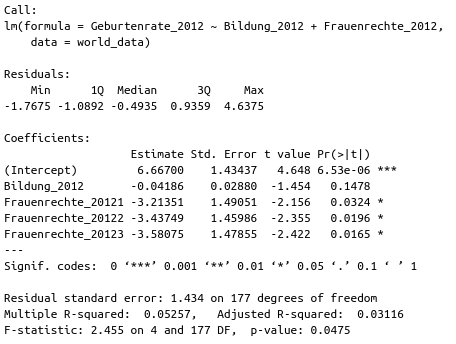
\includegraphics[scale=0.3]{../Plots/sum_multi.png}
      \end{minipage}%
      \begin{minipage}[t]{0.45\textwidth}
        \vspace{-1em}

        \centering
        \begin{lstlisting}
library(relaimpo)
calc.relimp(model_multi, type="lmg",rela=T,rank=T)    
                  \end{lstlisting} 

        % %\vspace{-1em}
        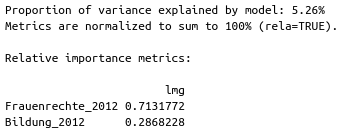
\includegraphics[scale=0.5]{../Plots/relimp_multi.png}
      \end{minipage}
  \end{frame}

%------------------
\section{Take Home Message}
%------------------
\setbeamertemplate{background canvas}[default]
\setbeamercolor{background canvas}{bg=PN3}
\thispagestyle{empty}
\begin{frame} 
\begin{center}
\textcolor{SS2}{\huge{\textbf{Take Home Message}}}
\end{center}
\end{frame}

\setbeamercolor{background canvas}{bg=}
    \begin{frame}[t]
      \begin{minipage}[t]{0.45\textwidth}
        \begin{itemize}
            \item[] \textbf{Zusammenfassung:}
            \item Regressionen als Mittel um Zusammenhänge zwischen einer oder mehrerer Variablen zu überprüfen
            \item Wahl der Regressionsart abhängig von:
            \begin{itemize}
              \footnotesize
              \item Art der Variablen
              \item Verteilung der Standardfehler
              \item Heteroskedastizität
              \item Multikolliniarität
            \end{itemize}
        \end{itemize}
        \scriptsize
        \begin{tcolorbox}[title=Achtung!, colframe=red!80!black, colback=orange!25]
          \centering
          Korrelation $\neq$ Kausalbeziehung
        \end{tcolorbox}
      \end{minipage}%
      \begin{minipage}[t]{0.45\textwidth}
        \begin{itemize}
          \item[] \textbf{Weiterführende Literatur:}
          \scriptsize  
          \item \fullcite{Hedderich2016} 
          \item \fullcite{Wolf2010}
          \item \fullcite{Ciaburro2018}
          \item \fullcite{Pardoe2020}
        \end{itemize}
      \end{minipage}
    \end{frame}
\end{document}